\graphicspath{{./figures}}

\section{Overview}

This project aims to design and implement a wireless communication system for a miniaturised satellite standard called a \textit{PocketQube} (PQ). The PocketQube standard was created to define physical and electronic requirements for so-called "nano satellites". The goal of this is to allow for easy integration of various sub-modules into one physical enclosure. One common use-case of these satellites is to collect sensory information from the atmosphere.

Nano-satellites can either be placed into orbit, or attached to a \textit{high-altitude balloon} as shown in Figure \ref{fig:balloonSat}. The goal of this project is to design a communication system that is compatible with the PocketQube standard. The final system should be capable of being used in a balloon satellite launch from the Saldanha Air Field in the Western Cape, which might be done by the Stellenbosch Engineering department near the end of the project.

\begin{figure}[!htb]
  \centering
  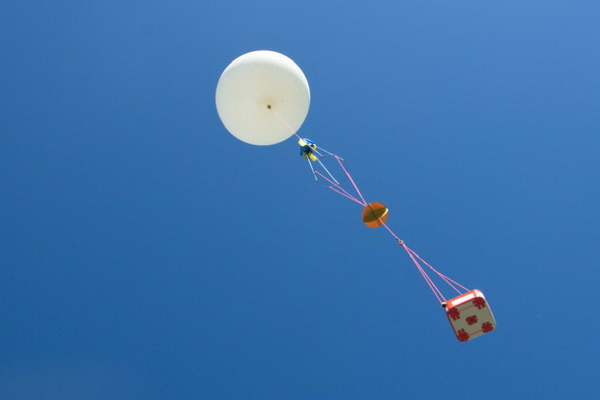
\includegraphics[width=0.5\textwidth]{balloonSat}
  \caption{A Balloon Satellite \cite{site-cyberBalloonLaunch}}
  \label{fig:balloonSat}
\end{figure}

Both higher-level systems design, as well as more detailed lower-level component selection, integration, and software design, will be necessary for this project. The communication system will involve both a tracking ground station (GS), as well as a PocketQube 'unit' (PQU). The aim of this project is to both design and implement this system, in order to establish a minimal baseline for further projects to refine the individual sub-systems. The GS should also be capable of receiving information from an existing \textit{Radiosonde} to provide a backup system.

In this report, general system requirements are first listed, and a problem statement is drawn up. Then, a literature review is conducted to gather background information in the fields of interest. This includes an overview of the PocketQube standard, antenna theory, satellite tracking, and telecommunication theory. A system's level design is then done, which is followed by a more detailed design. Finally, the system is implemented and tested, and the results are discussed, and potential improvements for future projects are listed.